\section{Pre-amplificatore}
	Per realizzare il pre-amplificatore è stato realizzato il circuito in 
	\figurename{ \ref{fig:ampli}} impiegando le corrispondenti componenti
	circuitali.
	
		\begin{figure}[h]
		\begin{minipage}{0.75\textwidth}
			\centering
			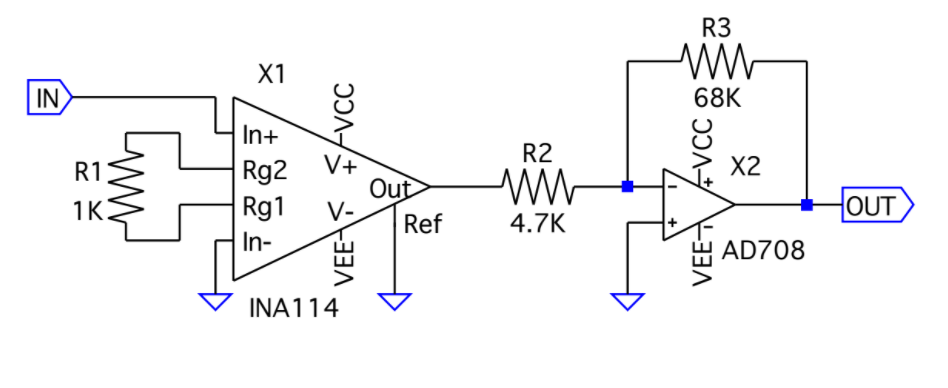
\includegraphics[width=\textwidth]{ampli.png}
			\caption{Circuito pre-amplificatore.}
			\label{fig:pre}
		\end{minipage}
		\begin{minipage}{0.19\textwidth}
			\begin{tabular}{l@{ }c@{ }l}
				$R_{1}$& = &\SI{0.971(9)}{\kilo\ohm}\\
				$R_{2}$& = &\SI{4.69(5)}{\kilo\ohm}\\
				$R_3$& = &\SI{71.9(7)}{\kilo\ohm}\\
			\end{tabular}
		\end{minipage}
	\end{figure}
	Essendo il un guadagno atteso in $out$ $\sim 51 \cdot 14.5 \sim 740$ per effettuare
	la verifica, evitando che l'uscita dell'op-amp saturi è stato montato un partitore di 
	Thevenen
	impiegando le resistenze $R_{T1}=$\SI{0.987(9)}{\kilo\ohm} $R_{T2}=$\SI{1031(9)}{\kilo\ohm}
	ottenendo pertanto un guadagno  $Av_{T}=0.00096 \pm 0.00001$.
	
	Si è proceduto pertanto ad inviare in ingresso al partitore un onda sinusoidale di 
	$V_{pp}=$\SI{21.0 (2)}{\volt}, ottenendo all'uscita $Ref$ un onda sinusoidale di ampiezza
	picco-picco $V_{ref}=$\SI{1.10 (1)}{\volt} (\figurename{ \ref{fig:preamp1}}).
	
		
	Il guadagno ottenuto $Av_{1}= 55 \pm 1$ risulta compatibile con le attese $\sim 51$.
	
	Effettuata questa prima verifica si è proceduto a verificare il guadagno della seconda
	parte del circuito montato, $Av_{2}= \frac{V_{out}}{V_{ref}}$.
	Essendo i due circuiti indipendenti è stato optato per non impiegare $V_{ref}$ data dall'uscita 
	del precedente op-amp
	ma un segnale sinusoidale generato esternamente, ottenendo i segnali riportati in
	\figurename{ \ref{fig:preamp2}}.
	Si ottengono per $V_{ref}=$\SI{0.374 (2)}{\volt} si ottiene un segnale in uscita
	$V_{out}=$\SI{5.68 (4)}{\volt} e pertanto un guadagno $Av_{2})=15.2 \pm 0.1$.
	Tale guadagno risulta compatibile coi valori attesi $\sim 14.5$.
	
	Il fatto che i guadagni misurati risultino maggiori di quelli previsti è stato imputato al 
	diverso valore dei resistori dai loro valori nominali.
	
		\begin{figure}[h]
		\begin{minipage}{0.45\textwidth}
			\centering
			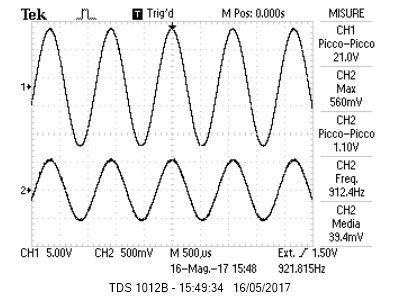
\includegraphics[scale=0.75]{preamp1.png}
			\caption{Acquisizione segnali in ingresso al partitore ch.1 e in $ref$ ch.2.}
			\label{fig:preamp1}
		\end{minipage}
		\begin{minipage}{0.45\textwidth}
			\centering
			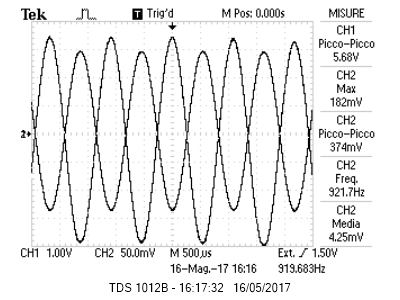
\includegraphics[scale=0.75]{preampb.png}
			\caption{Acquisizione segnali in ingresso ch.1 e in $out$ ch.2.}
			\label{fig:preamp2}
		\end{minipage}
	\end{figure}
	
	